\documentclass[1p]{elsarticle_modified}
%\bibliographystyle{elsarticle-num}

%\usepackage[colorlinks]{hyperref}
%\usepackage{abbrmath_seonhwa} %\Abb, \Ascr, \Acal ,\Abf, \Afrak
\usepackage{amsfonts}
\usepackage{amssymb}
\usepackage{amsmath}
\usepackage{amsthm}
\usepackage{scalefnt}
\usepackage{amsbsy}
\usepackage{kotex}
\usepackage{caption}
\usepackage{subfig}
\usepackage{color}
\usepackage{graphicx}
\usepackage{xcolor} %% white, black, red, green, blue, cyan, magenta, yellow
\usepackage{float}
\usepackage{setspace}
\usepackage{hyperref}

\usepackage{tikz}
\usetikzlibrary{arrows}

\usepackage{multirow}
\usepackage{array} % fixed length table
\usepackage{hhline}

%%%%%%%%%%%%%%%%%%%%%
\makeatletter
\renewcommand*\env@matrix[1][\arraystretch]{%
	\edef\arraystretch{#1}%
	\hskip -\arraycolsep
	\let\@ifnextchar\new@ifnextchar
	\array{*\c@MaxMatrixCols c}}
\makeatother %https://tex.stackexchange.com/questions/14071/how-can-i-increase-the-line-spacing-in-a-matrix
%%%%%%%%%%%%%%%

\usepackage[normalem]{ulem}

\newcommand{\msout}[1]{\ifmmode\text{\sout{\ensuremath{#1}}}\else\sout{#1}\fi}
%SOURCE: \msout is \stkout macro in https://tex.stackexchange.com/questions/20609/strikeout-in-math-mode

\newcommand{\cancel}[1]{
	\ifmmode
	{\color{red}\msout{#1}}
	\else
	{\color{red}\sout{#1}}
	\fi
}

\newcommand{\add}[1]{
	{\color{blue}\uwave{#1}}
}

\newcommand{\replace}[2]{
	\ifmmode
	{\color{red}\msout{#1}}{\color{blue}\uwave{#2}}
	\else
	{\color{red}\sout{#1}}{\color{blue}\uwave{#2}}
	\fi
}

\newcommand{\Sol}{\mathcal{S}} %segment
\newcommand{\D}{D} %diagram
\newcommand{\A}{\mathcal{A}} %arc


%%%%%%%%%%%%%%%%%%%%%%%%%%%%%5 test

\def\sl{\operatorname{\textup{SL}}(2,\Cbb)}
\def\psl{\operatorname{\textup{PSL}}(2,\Cbb)}
\def\quan{\mkern 1mu \triangleright \mkern 1mu}

\theoremstyle{definition}
\newtheorem{thm}{Theorem}[section]
\newtheorem{prop}[thm]{Proposition}
\newtheorem{lem}[thm]{Lemma}
\newtheorem{ques}[thm]{Question}
\newtheorem{cor}[thm]{Corollary}
\newtheorem{defn}[thm]{Definition}
\newtheorem{exam}[thm]{Example}
\newtheorem{rmk}[thm]{Remark}
\newtheorem{alg}[thm]{Algorithm}

\newcommand{\I}{\sqrt{-1}}
\begin{document}

%\begin{frontmatter}
%
%\title{Boundary parabolic representations of knots up to 8 crossings}
%
%%% Group authors per affiliation:
%\author{Yunhi Cho} 
%\address{Department of Mathematics, University of Seoul, Seoul, Korea}
%\ead{yhcho@uos.ac.kr}
%
%
%\author{Seonhwa Kim} %\fnref{s_kim}}
%\address{Center for Geometry and Physics, Institute for Basic Science, Pohang, 37673, Korea}
%\ead{ryeona17@ibs.re.kr}
%
%\author{Hyuk Kim}
%\address{Department of Mathematical Sciences, Seoul National University, Seoul 08826, Korea}
%\ead{hyukkim@snu.ac.kr}
%
%\author{Seokbeom Yoon}
%\address{Department of Mathematical Sciences, Seoul National University, Seoul, 08826,  Korea}
%\ead{sbyoon15@snu.ac.kr}
%
%\begin{abstract}
%We find all boundary parabolic representation of knots up to 8 crossings.
%
%\end{abstract}
%\begin{keyword}
%    \MSC[2010] 57M25 
%\end{keyword}
%
%\end{frontmatter}

%\linenumbers
%\tableofcontents
%
\newcommand\colored[1]{\textcolor{white}{\rule[-0.35ex]{0.8em}{1.4ex}}\kern-0.8em\color{red} #1}%
%\newcommand\colored[1]{\textcolor{white}{ #1}\kern-2.17ex	\textcolor{white}{ #1}\kern-1.81ex	\textcolor{white}{ #1}\kern-2.15ex\color{red}#1	}

{\Large $\underline{12n_{0301}~(K12n_{0301})}$}

\setlength{\tabcolsep}{10pt}
\renewcommand{\arraystretch}{1.6}
\vspace{1cm}\begin{tabular}{m{100pt}>{\centering\arraybackslash}m{274pt}}
\multirow{5}{120pt}{
	\centering
	\includegraphics[width=112pt]{../../../GIT/diagram.site/Diagrams/png/2390_12n_0301.png}\\
\ \ \ A knot diagram\footnotemark}&
\allowdisplaybreaks
\textbf{Linearized knot diagam} \\
\cline{2-2}
 &
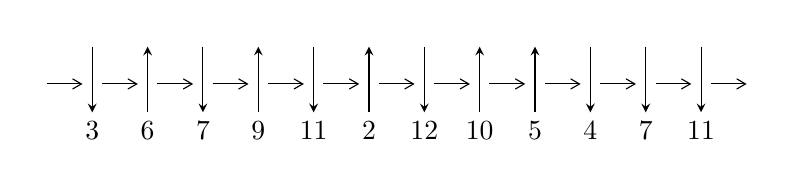
\begin{tikzpicture}[x=20pt, y=17pt]
	% nodes
	\node (C0) at (0, 0) {};
	\node (C1) at (1, 0) {};
	\node (C1U) at (1, +1) {};
	\node (C1D) at (1, -1) {3};

	\node (C2) at (2, 0) {};
	\node (C2U) at (2, +1) {};
	\node (C2D) at (2, -1) {6};

	\node (C3) at (3, 0) {};
	\node (C3U) at (3, +1) {};
	\node (C3D) at (3, -1) {7};

	\node (C4) at (4, 0) {};
	\node (C4U) at (4, +1) {};
	\node (C4D) at (4, -1) {9};

	\node (C5) at (5, 0) {};
	\node (C5U) at (5, +1) {};
	\node (C5D) at (5, -1) {11};

	\node (C6) at (6, 0) {};
	\node (C6U) at (6, +1) {};
	\node (C6D) at (6, -1) {2};

	\node (C7) at (7, 0) {};
	\node (C7U) at (7, +1) {};
	\node (C7D) at (7, -1) {12};

	\node (C8) at (8, 0) {};
	\node (C8U) at (8, +1) {};
	\node (C8D) at (8, -1) {10};

	\node (C9) at (9, 0) {};
	\node (C9U) at (9, +1) {};
	\node (C9D) at (9, -1) {5};

	\node (C10) at (10, 0) {};
	\node (C10U) at (10, +1) {};
	\node (C10D) at (10, -1) {4};

	\node (C11) at (11, 0) {};
	\node (C11U) at (11, +1) {};
	\node (C11D) at (11, -1) {7};

	\node (C12) at (12, 0) {};
	\node (C12U) at (12, +1) {};
	\node (C12D) at (12, -1) {11};
	\node (C13) at (13, 0) {};

	% arrows
	\draw[->,>={angle 60}]
	(C0) edge (C1) (C1) edge (C2) (C2) edge (C3) (C3) edge (C4) (C4) edge (C5) (C5) edge (C6) (C6) edge (C7) (C7) edge (C8) (C8) edge (C9) (C9) edge (C10) (C10) edge (C11) (C11) edge (C12) (C12) edge (C13) ;	\draw[->,>=stealth]
	(C1U) edge (C1D) (C2D) edge (C2U) (C3U) edge (C3D) (C4D) edge (C4U) (C5U) edge (C5D) (C6D) edge (C6U) (C7U) edge (C7D) (C8D) edge (C8U) (C9D) edge (C9U) (C10U) edge (C10D) (C11U) edge (C11D) (C12U) edge (C12D) ;
	\end{tikzpicture} \\
\hhline{~~} \\& 
\textbf{Solving Sequence} \\ \cline{2-2} 
 &
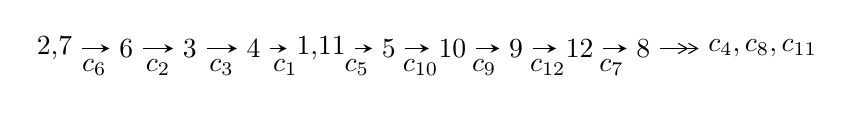
\begin{tikzpicture}[x=23pt, y=7pt]
	% node
	\node (A0) at (-1/8, 0) {2,7};
	\node (A1) at (1, 0) {6};
	\node (A2) at (2, 0) {3};
	\node (A3) at (3, 0) {4};
	\node (A4) at (65/16, 0) {1,11};
	\node (A5) at (41/8, 0) {5};
	\node (A6) at (49/8, 0) {10};
	\node (A7) at (57/8, 0) {9};
	\node (A8) at (65/8, 0) {12};
	\node (A9) at (73/8, 0) {8};
	\node (C1) at (1/2, -1) {$c_{6}$};
	\node (C2) at (3/2, -1) {$c_{2}$};
	\node (C3) at (5/2, -1) {$c_{3}$};
	\node (C4) at (7/2, -1) {$c_{1}$};
	\node (C5) at (37/8, -1) {$c_{5}$};
	\node (C6) at (45/8, -1) {$c_{10}$};
	\node (C7) at (53/8, -1) {$c_{9}$};
	\node (C8) at (61/8, -1) {$c_{12}$};
	\node (C9) at (69/8, -1) {$c_{7}$};
	\node (A10) at (11, 0) {$c_{4},c_{8},c_{11}$};

	% edge
	\draw[->,>=stealth]	
	(A0) edge (A1) (A1) edge (A2) (A2) edge (A3) (A3) edge (A4) (A4) edge (A5) (A5) edge (A6) (A6) edge (A7) (A7) edge (A8) (A8) edge (A9) ;
	\draw[->>,>={angle 60}]	
	(A9) edge (A10);
\end{tikzpicture} \\ 

\end{tabular} \\

\footnotetext{
The image of knot diagram is generated by the software ``\textbf{Draw programme}" developed by Andrew Bartholomew(\url{http://www.layer8.co.uk/maths/draw/index.htm\#Running-draw}), where we modified some parts for our purpose(\url{https://github.com/CATsTAILs/LinksPainter}).
}\phantom \\ \newline 
\centering \textbf{Ideals for irreducible components\footnotemark of $X_{\text{par}}$} 
 
\begin{align*}
I^u_{1}&=\langle 
1.34577\times10^{36} u^{46}+4.13410\times10^{36} u^{45}+\cdots+6.18526\times10^{36} b+7.22944\times10^{36},\\
\phantom{I^u_{1}}&\phantom{= \langle  }-4.63131\times10^{36} u^{46}-3.13332\times10^{37} u^{45}+\cdots+6.18526\times10^{37} a-1.27145\times10^{38},\;u^{47}+2 u^{46}+\cdots-7 u^2+5\rangle \\
I^u_{2}&=\langle 
b+1,\;a^4+4 a^3 u-8 a^2 u-8 a^2+8 a+5 u,\;u^2+u+1\rangle \\
I^u_{3}&=\langle 
b-1,\;a^3+3 a^2 u+3 a u-3 a-1,\;u^2- u+1\rangle \\
\\
\end{align*}
\raggedright * 3 irreducible components of $\dim_{\mathbb{C}}=0$, with total 61 representations.\\
\footnotetext{All coefficients of polynomials are rational numbers. But the coefficients are sometimes approximated in decimal forms when there is not enough margin.}
\newpage
\renewcommand{\arraystretch}{1}
\centering \section*{I. $I^u_{1}= \langle 1.35\times10^{36} u^{46}+4.13\times10^{36} u^{45}+\cdots+6.19\times10^{36} b+7.23\times10^{36},\;-4.63\times10^{36} u^{46}-3.13\times10^{37} u^{45}+\cdots+6.19\times10^{37} a-1.27\times10^{38},\;u^{47}+2 u^{46}+\cdots-7 u^2+5 \rangle$}
\flushleft \textbf{(i) Arc colorings}\\
\begin{tabular}{m{7pt} m{180pt} m{7pt} m{180pt} }
\flushright $a_{2}=$&$\begin{pmatrix}0\\u\end{pmatrix}$ \\
\flushright $a_{7}=$&$\begin{pmatrix}1\\0\end{pmatrix}$ \\
\flushright $a_{6}=$&$\begin{pmatrix}1\\u^2\end{pmatrix}$ \\
\flushright $a_{3}=$&$\begin{pmatrix}u\\u^3+u\end{pmatrix}$ \\
\flushright $a_{4}=$&$\begin{pmatrix}- u^3\\u^3+u\end{pmatrix}$ \\
\flushright $a_{1}=$&$\begin{pmatrix}u^3\\u^5+u^3+u\end{pmatrix}$ \\
\flushright $a_{11}=$&$\begin{pmatrix}0.0748766 u^{46}+0.506578 u^{45}+\cdots-0.0189566 u+2.05560\\-0.217577 u^{46}-0.668379 u^{45}+\cdots+0.153362 u-1.16882\end{pmatrix}$ \\
\flushright $a_{5}=$&$\begin{pmatrix}0.371873 u^{46}+0.438846 u^{45}+\cdots+1.29351 u+0.575382\\-0.151221 u^{46}-0.179133 u^{45}+\cdots-1.44030 u+0.207091\end{pmatrix}$ \\
\flushright $a_{10}=$&$\begin{pmatrix}0.234371 u^{46}+1.04621 u^{45}+\cdots+0.637032 u+2.96733\\-0.245873 u^{46}-0.763265 u^{45}+\cdots-0.314870 u-1.29989\end{pmatrix}$ \\
\flushright $a_{9}=$&$\begin{pmatrix}-0.0256670 u^{46}-0.692390 u^{45}+\cdots-1.49667 u-3.70685\\0.0370363 u^{46}+0.134133 u^{45}+\cdots+1.12375 u+0.747882\end{pmatrix}$ \\
\flushright $a_{12}=$&$\begin{pmatrix}0.292454 u^{46}+1.17496 u^{45}+\cdots-0.172319 u+3.22442\\-0.217577 u^{46}-0.668379 u^{45}+\cdots+0.153362 u-1.16882\end{pmatrix}$ \\
\flushright $a_{8}=$&$\begin{pmatrix}-0.187891 u^{46}-0.374761 u^{45}+\cdots+0.526224 u+0.0784946\\0.216050 u^{46}+0.341229 u^{45}+\cdots+1.29950 u+0.242159\end{pmatrix}$\\&\end{tabular}
\flushleft \textbf{(ii) Obstruction class $= -1$}\\~\\
\flushleft \textbf{(iii) Cusp Shapes $= 0.884631 u^{46}+2.37548 u^{45}+\cdots+0.300832 u+0.344938$}\\~\\
\newpage\renewcommand{\arraystretch}{1}
\flushleft \textbf{(iv) u-Polynomials at the component}\newline \\
\begin{tabular}{m{50pt}|m{274pt}}
Crossings & \hspace{64pt}u-Polynomials at each crossing \\
\hline $$\begin{aligned}c_{1}\end{aligned}$$&$\begin{aligned}
&u^{47}+30 u^{46}+\cdots+70 u-25
\end{aligned}$\\
\hline $$\begin{aligned}c_{2},c_{6}\end{aligned}$$&$\begin{aligned}
&u^{47}-2 u^{46}+\cdots+7 u^2-5
\end{aligned}$\\
\hline $$\begin{aligned}c_{3}\end{aligned}$$&$\begin{aligned}
&u^{47}+2 u^{46}+\cdots+20 u-5
\end{aligned}$\\
\hline $$\begin{aligned}c_{4},c_{9}\end{aligned}$$&$\begin{aligned}
&u^{47}+u^{46}+\cdots+12 u+4
\end{aligned}$\\
\hline $$\begin{aligned}c_{5}\end{aligned}$$&$\begin{aligned}
&u^{47}- u^{46}+\cdots+36 u+4
\end{aligned}$\\
\hline $$\begin{aligned}c_{7},c_{11}\end{aligned}$$&$\begin{aligned}
&u^{47}+3 u^{46}+\cdots-29 u+1
\end{aligned}$\\
\hline $$\begin{aligned}c_{8}\end{aligned}$$&$\begin{aligned}
&u^{47}-21 u^{46}+\cdots+80 u-16
\end{aligned}$\\
\hline $$\begin{aligned}c_{10}\end{aligned}$$&$\begin{aligned}
&u^{47}+3 u^{46}+\cdots-1940 u-172
\end{aligned}$\\
\hline $$\begin{aligned}c_{12}\end{aligned}$$&$\begin{aligned}
&u^{47}+63 u^{46}+\cdots+175 u+1
\end{aligned}$\\
\hline
\end{tabular}\\~\\
\newpage\renewcommand{\arraystretch}{1}
\flushleft \textbf{(v) Riley Polynomials at the component}\newline \\
\begin{tabular}{m{50pt}|m{274pt}}
Crossings & \hspace{64pt}Riley Polynomials at each crossing \\
\hline $$\begin{aligned}c_{1}\end{aligned}$$&$\begin{aligned}
&y^{47}-18 y^{46}+\cdots+2450 y-625
\end{aligned}$\\
\hline $$\begin{aligned}c_{2},c_{6}\end{aligned}$$&$\begin{aligned}
&y^{47}+30 y^{46}+\cdots+70 y-25
\end{aligned}$\\
\hline $$\begin{aligned}c_{3}\end{aligned}$$&$\begin{aligned}
&y^{47}-66 y^{46}+\cdots-330 y-25
\end{aligned}$\\
\hline $$\begin{aligned}c_{4},c_{9}\end{aligned}$$&$\begin{aligned}
&y^{47}-21 y^{46}+\cdots+80 y-16
\end{aligned}$\\
\hline $$\begin{aligned}c_{5}\end{aligned}$$&$\begin{aligned}
&y^{47}-69 y^{46}+\cdots-112 y-16
\end{aligned}$\\
\hline $$\begin{aligned}c_{7},c_{11}\end{aligned}$$&$\begin{aligned}
&y^{47}-63 y^{46}+\cdots+175 y-1
\end{aligned}$\\
\hline $$\begin{aligned}c_{8}\end{aligned}$$&$\begin{aligned}
&y^{47}+15 y^{46}+\cdots+256 y-256
\end{aligned}$\\
\hline $$\begin{aligned}c_{10}\end{aligned}$$&$\begin{aligned}
&y^{47}-9 y^{46}+\cdots+1462928 y-29584
\end{aligned}$\\
\hline $$\begin{aligned}c_{12}\end{aligned}$$&$\begin{aligned}
&y^{47}-143 y^{46}+\cdots+12319 y-1
\end{aligned}$\\
\hline
\end{tabular}\\~\\
\newpage\flushleft \textbf{(vi) Complex Volumes and Cusp Shapes}
$$\begin{array}{c|c|c}  
\text{Solutions to }I^u_{1}& \I (\text{vol} + \sqrt{-1}CS) & \text{Cusp shape}\\
 \hline 
\begin{aligned}
u &= \phantom{-}0.520853 + 0.848466 I \\
a &= -1.084380 + 0.109048 I \\
b &= -0.0925902 + 0.0236889 I\end{aligned}
 & \phantom{-}2.45436 + 5.70987 I & \phantom{-}4.10397 - 7.52673 I \\ \hline\begin{aligned}
u &= \phantom{-}0.520853 - 0.848466 I \\
a &= -1.084380 - 0.109048 I \\
b &= -0.0925902 - 0.0236889 I\end{aligned}
 & \phantom{-}2.45436 - 5.70987 I & \phantom{-}4.10397 + 7.52673 I \\ \hline\begin{aligned}
u &= -0.954753\phantom{ +0.000000I} \\
a &= -0.462105\phantom{ +0.000000I} \\
b &= \phantom{-}1.61809\phantom{ +0.000000I}\end{aligned}
 & -4.77856\phantom{ +0.000000I} & -0.0822940\phantom{ +0.000000I} \\ \hline\begin{aligned}
u &= -0.426277 + 0.843973 I \\
a &= \phantom{-}0.695944 + 0.007832 I \\
b &= -0.126186 + 0.180791 I\end{aligned}
 & -0.08833 - 1.82304 I & -0.21214 + 3.66824 I \\ \hline\begin{aligned}
u &= -0.426277 - 0.843973 I \\
a &= \phantom{-}0.695944 - 0.007832 I \\
b &= -0.126186 - 0.180791 I\end{aligned}
 & -0.08833 + 1.82304 I & -0.21214 - 3.66824 I \\ \hline\begin{aligned}
u &= \phantom{-}0.080676 + 1.062940 I \\
a &= \phantom{-}2.21302 - 0.62081 I \\
b &= -1.251550 - 0.323161 I\end{aligned}
 & -1.26187 + 4.11733 I & -5.79211 - 3.02419 I \\ \hline\begin{aligned}
u &= \phantom{-}0.080676 - 1.062940 I \\
a &= \phantom{-}2.21302 + 0.62081 I \\
b &= -1.251550 + 0.323161 I\end{aligned}
 & -1.26187 - 4.11733 I & -5.79211 + 3.02419 I \\ \hline\begin{aligned}
u &= -1.065870 + 0.151558 I \\
a &= -0.220607 - 0.235501 I \\
b &= \phantom{-}1.73800 - 0.19985 I\end{aligned}
 & -9.19783 + 7.78492 I & -3.11194 - 4.36379 I \\ \hline\begin{aligned}
u &= -1.065870 - 0.151558 I \\
a &= -0.220607 + 0.235501 I \\
b &= \phantom{-}1.73800 + 0.19985 I\end{aligned}
 & -9.19783 - 7.78492 I & -3.11194 + 4.36379 I \\ \hline\begin{aligned}
u &= \phantom{-}1.074670 + 0.087030 I \\
a &= \phantom{-}0.234458 - 0.134402 I \\
b &= -1.76123 - 0.11585 I\end{aligned}
 & -11.04170 - 2.07575 I & -5.37324 + 0.07581 I\\
 \hline 
 \end{array}$$\newpage$$\begin{array}{c|c|c}  
\text{Solutions to }I^u_{1}& \I (\text{vol} + \sqrt{-1}CS) & \text{Cusp shape}\\
 \hline 
\begin{aligned}
u &= \phantom{-}1.074670 - 0.087030 I \\
a &= \phantom{-}0.234458 + 0.134402 I \\
b &= -1.76123 + 0.11585 I\end{aligned}
 & -11.04170 + 2.07575 I & -5.37324 - 0.07581 I \\ \hline\begin{aligned}
u &= -0.416939 + 1.002100 I \\
a &= \phantom{-}1.021110 - 0.519987 I \\
b &= -0.564053 - 0.373274 I\end{aligned}
 & -0.35308 - 2.84906 I & \phantom{-}0.14660 + 5.36409 I \\ \hline\begin{aligned}
u &= -0.416939 - 1.002100 I \\
a &= \phantom{-}1.021110 + 0.519987 I \\
b &= -0.564053 + 0.373274 I\end{aligned}
 & -0.35308 + 2.84906 I & \phantom{-}0.14660 - 5.36409 I \\ \hline\begin{aligned}
u &= \phantom{-}0.045591 + 1.099550 I \\
a &= -1.79233 - 0.59931 I \\
b &= \phantom{-}1.189770 - 0.444997 I\end{aligned}
 & -3.94139 + 0.69325 I & -8.93702 - 1.07384 I \\ \hline\begin{aligned}
u &= \phantom{-}0.045591 - 1.099550 I \\
a &= -1.79233 + 0.59931 I \\
b &= \phantom{-}1.189770 + 0.444997 I\end{aligned}
 & -3.94139 - 0.69325 I & -8.93702 + 1.07384 I \\ \hline\begin{aligned}
u &= \phantom{-}0.514947 + 0.719739 I \\
a &= -0.652546 + 0.529793 I \\
b &= -0.095652 + 0.345286 I\end{aligned}
 & \phantom{-}2.80273 - 1.43971 I & \phantom{-}4.88073 + 0.31816 I \\ \hline\begin{aligned}
u &= \phantom{-}0.514947 - 0.719739 I \\
a &= -0.652546 - 0.529793 I \\
b &= -0.095652 - 0.345286 I\end{aligned}
 & \phantom{-}2.80273 + 1.43971 I & \phantom{-}4.88073 - 0.31816 I \\ \hline\begin{aligned}
u &= \phantom{-}0.606629 + 0.637775 I \\
a &= -0.221188 - 1.122120 I \\
b &= \phantom{-}1.161630 - 0.221796 I\end{aligned}
 & -1.182870 + 0.647616 I & -3.09275 + 0.88493 I \\ \hline\begin{aligned}
u &= \phantom{-}0.606629 - 0.637775 I \\
a &= -0.221188 + 1.122120 I \\
b &= \phantom{-}1.161630 + 0.221796 I\end{aligned}
 & -1.182870 - 0.647616 I & -3.09275 - 0.88493 I \\ \hline\begin{aligned}
u &= -0.091353 + 1.151430 I \\
a &= \phantom{-}0.063117 - 0.348259 I \\
b &= -0.154148 + 0.895743 I\end{aligned}
 & -2.52743 - 2.40559 I & -6.04313 + 3.27210 I\\
 \hline 
 \end{array}$$\newpage$$\begin{array}{c|c|c}  
\text{Solutions to }I^u_{1}& \I (\text{vol} + \sqrt{-1}CS) & \text{Cusp shape}\\
 \hline 
\begin{aligned}
u &= -0.091353 - 1.151430 I \\
a &= \phantom{-}0.063117 + 0.348259 I \\
b &= -0.154148 - 0.895743 I\end{aligned}
 & -2.52743 + 2.40559 I & -6.04313 - 3.27210 I \\ \hline\begin{aligned}
u &= -0.067124 + 0.804789 I \\
a &= \phantom{-}1.56336 - 1.49824 I \\
b &= -1.064520 - 0.261047 I\end{aligned}
 & -0.09852 - 3.64662 I & -4.05106 + 4.37055 I \\ \hline\begin{aligned}
u &= -0.067124 - 0.804789 I \\
a &= \phantom{-}1.56336 + 1.49824 I \\
b &= -1.064520 + 0.261047 I\end{aligned}
 & -0.09852 + 3.64662 I & -4.05106 - 4.37055 I \\ \hline\begin{aligned}
u &= \phantom{-}0.688119 + 0.988855 I \\
a &= -0.236313 - 0.766691 I \\
b &= \phantom{-}1.328370 + 0.259774 I\end{aligned}
 & -2.22622 + 4.49419 I & -5.40692 - 5.46385 I \\ \hline\begin{aligned}
u &= \phantom{-}0.688119 - 0.988855 I \\
a &= -0.236313 + 0.766691 I \\
b &= \phantom{-}1.328370 - 0.259774 I\end{aligned}
 & -2.22622 - 4.49419 I & -5.40692 + 5.46385 I \\ \hline\begin{aligned}
u &= -0.586580 + 1.068360 I \\
a &= \phantom{-}0.267571 - 0.668867 I \\
b &= -1.138940 + 0.454251 I\end{aligned}
 & -2.43118 - 0.00318 I & -6.09049 + 0. I\phantom{ +0.000000I} \\ \hline\begin{aligned}
u &= -0.586580 - 1.068360 I \\
a &= \phantom{-}0.267571 + 0.668867 I \\
b &= -1.138940 - 0.454251 I\end{aligned}
 & -2.43118 + 0.00318 I & -6.09049 + 0. I\phantom{ +0.000000I} \\ \hline\begin{aligned}
u &= \phantom{-}0.290782 + 1.240950 I \\
a &= -1.325260 - 0.374001 I \\
b &= \phantom{-}0.985287 - 0.825561 I\end{aligned}
 & -5.50399 + 3.13913 I & \phantom{-0.000000 } 0 \\ \hline\begin{aligned}
u &= \phantom{-}0.290782 - 1.240950 I \\
a &= -1.325260 + 0.374001 I \\
b &= \phantom{-}0.985287 + 0.825561 I\end{aligned}
 & -5.50399 - 3.13913 I & \phantom{-0.000000 } 0 \\ \hline\begin{aligned}
u &= -0.377179 + 1.257740 I \\
a &= \phantom{-}1.235730 - 0.352288 I \\
b &= -0.848401 - 0.946720 I\end{aligned}
 & -4.21139 - 8.46222 I & \phantom{-0.000000 } 0\\
 \hline 
 \end{array}$$\newpage$$\begin{array}{c|c|c}  
\text{Solutions to }I^u_{1}& \I (\text{vol} + \sqrt{-1}CS) & \text{Cusp shape}\\
 \hline 
\begin{aligned}
u &= -0.377179 - 1.257740 I \\
a &= \phantom{-}1.235730 + 0.352288 I \\
b &= -0.848401 + 0.946720 I\end{aligned}
 & -4.21139 + 8.46222 I & \phantom{-0.000000 } 0 \\ \hline\begin{aligned}
u &= -0.672082 + 0.139197 I \\
a &= -0.260444 - 1.022400 I \\
b &= -0.842370 - 0.552537 I\end{aligned}
 & -0.14779 - 4.58136 I & -1.59423 + 6.34344 I \\ \hline\begin{aligned}
u &= -0.672082 - 0.139197 I \\
a &= -0.260444 + 1.022400 I \\
b &= -0.842370 + 0.552537 I\end{aligned}
 & -0.14779 + 4.58136 I & -1.59423 - 6.34344 I \\ \hline\begin{aligned}
u &= -0.498424 + 1.300460 I \\
a &= -1.83978 + 1.10496 I \\
b &= \phantom{-}1.71077 + 0.16414 I\end{aligned}
 & -8.75756 - 5.17554 I & \phantom{-0.000000 } 0 \\ \hline\begin{aligned}
u &= -0.498424 - 1.300460 I \\
a &= -1.83978 - 1.10496 I \\
b &= \phantom{-}1.71077 - 0.16414 I\end{aligned}
 & -8.75756 + 5.17554 I & \phantom{-0.000000 } 0 \\ \hline\begin{aligned}
u &= -0.505508 + 0.300306 I \\
a &= -0.075783 + 0.611800 I \\
b &= -0.255894 + 0.505093 I\end{aligned}
 & \phantom{-}1.57367 - 0.84058 I & \phantom{-}3.87048 + 1.10428 I \\ \hline\begin{aligned}
u &= -0.505508 - 0.300306 I \\
a &= -0.075783 - 0.611800 I \\
b &= -0.255894 - 0.505093 I\end{aligned}
 & \phantom{-}1.57367 + 0.84058 I & \phantom{-}3.87048 - 1.10428 I \\ \hline\begin{aligned}
u &= -0.59657 + 1.30838 I \\
a &= -1.57480 + 1.26494 I \\
b &= \phantom{-}1.74692 + 0.35404 I\end{aligned}
 & -12.7785 - 13.7242 I & \phantom{-0.000000 } 0 \\ \hline\begin{aligned}
u &= -0.59657 - 1.30838 I \\
a &= -1.57480 - 1.26494 I \\
b &= \phantom{-}1.74692 - 0.35404 I\end{aligned}
 & -12.7785 + 13.7242 I & \phantom{-0.000000 } 0 \\ \hline\begin{aligned}
u &= \phantom{-}0.56882 + 1.33488 I \\
a &= \phantom{-}1.60835 + 1.16120 I \\
b &= -1.79435 + 0.29240 I\end{aligned}
 & -14.9238 + 7.9344 I & \phantom{-0.000000 } 0\\
 \hline 
 \end{array}$$\newpage$$\begin{array}{c|c|c}  
\text{Solutions to }I^u_{1}& \I (\text{vol} + \sqrt{-1}CS) & \text{Cusp shape}\\
 \hline 
\begin{aligned}
u &= \phantom{-}0.56882 - 1.33488 I \\
a &= \phantom{-}1.60835 - 1.16120 I \\
b &= -1.79435 - 0.29240 I\end{aligned}
 & -14.9238 - 7.9344 I & \phantom{-0.000000 } 0 \\ \hline\begin{aligned}
u &= -0.40822 + 1.40970 I \\
a &= -1.72088 + 0.73531 I \\
b &= \phantom{-}1.88085 - 0.04240 I\end{aligned}
 & -14.2777 + 2.5683 I & \phantom{-0.000000 } 0 \\ \hline\begin{aligned}
u &= -0.40822 - 1.40970 I \\
a &= -1.72088 - 0.73531 I \\
b &= \phantom{-}1.88085 + 0.04240 I\end{aligned}
 & -14.2777 - 2.5683 I & \phantom{-0.000000 } 0 \\ \hline\begin{aligned}
u &= \phantom{-}0.46183 + 1.39829 I \\
a &= \phantom{-}1.68707 + 0.85628 I \\
b &= -1.88332 + 0.06316 I\end{aligned}
 & -15.7940 + 3.3870 I & \phantom{-0.000000 } 0 \\ \hline\begin{aligned}
u &= \phantom{-}0.46183 - 1.39829 I \\
a &= \phantom{-}1.68707 - 0.85628 I \\
b &= -1.88332 - 0.06316 I\end{aligned}
 & -15.7940 - 3.3870 I & \phantom{-0.000000 } 0 \\ \hline\begin{aligned}
u &= \phantom{-}0.336586 + 0.137208 I \\
a &= \phantom{-}1.14561 - 1.39055 I \\
b &= \phantom{-}0.822565 - 0.188238 I\end{aligned}
 & -1.43951 + 0.37029 I & -6.25580 - 0.44865 I \\ \hline\begin{aligned}
u &= \phantom{-}0.336586 - 0.137208 I \\
a &= \phantom{-}1.14561 + 1.39055 I \\
b &= \phantom{-}0.822565 + 0.188238 I\end{aligned}
 & -1.43951 - 0.37029 I & -6.25580 + 0.44865 I\\
 \hline 
 \end{array}$$\newpage\newpage\renewcommand{\arraystretch}{1}
\centering \section*{II. $I^u_{2}= \langle b+1,\;a^4+4 a^3 u-8 a^2 u-8 a^2+8 a+5 u,\;u^2+u+1 \rangle$}
\flushleft \textbf{(i) Arc colorings}\\
\begin{tabular}{m{7pt} m{180pt} m{7pt} m{180pt} }
\flushright $a_{2}=$&$\begin{pmatrix}0\\u\end{pmatrix}$ \\
\flushright $a_{7}=$&$\begin{pmatrix}1\\0\end{pmatrix}$ \\
\flushright $a_{6}=$&$\begin{pmatrix}1\\- u-1\end{pmatrix}$ \\
\flushright $a_{3}=$&$\begin{pmatrix}u\\u+1\end{pmatrix}$ \\
\flushright $a_{4}=$&$\begin{pmatrix}-1\\u+1\end{pmatrix}$ \\
\flushright $a_{1}=$&$\begin{pmatrix}1\\0\end{pmatrix}$ \\
\flushright $a_{11}=$&$\begin{pmatrix}a\\-1\end{pmatrix}$ \\
\flushright $a_{5}=$&$\begin{pmatrix}- a^2 u- a^2+a+1\\a u+a- u-2\end{pmatrix}$ \\
\flushright $a_{10}=$&$\begin{pmatrix}a u+2 a-1\\- a u+u\end{pmatrix}$ \\
\flushright $a_{9}=$&$\begin{pmatrix}- a^3 u+a^3+5 a^2 u+2 a^2-3 a u-5 a+1\\- a^3 u- a^3+a^2 u+3 a^2+a u-2 a- u+1\end{pmatrix}$ \\
\flushright $a_{12}=$&$\begin{pmatrix}a+1\\-1\end{pmatrix}$ \\
\flushright $a_{8}=$&$\begin{pmatrix}- a\\1\end{pmatrix}$\\&\end{tabular}
\flushleft \textbf{(ii) Obstruction class $= 1$}\\~\\
\flushleft \textbf{(iii) Cusp Shapes $= 4 a^2 u-8 a u-8 a+4 u+8$}\\~\\
\newpage\renewcommand{\arraystretch}{1}
\flushleft \textbf{(iv) u-Polynomials at the component}\newline \\
\begin{tabular}{m{50pt}|m{274pt}}
Crossings & \hspace{64pt}u-Polynomials at each crossing \\
\hline $$\begin{aligned}c_{1},c_{2}\end{aligned}$$&$\begin{aligned}
&(u^2- u+1)^4
\end{aligned}$\\
\hline $$\begin{aligned}c_{3},c_{6}\end{aligned}$$&$\begin{aligned}
&(u^2+u+1)^4
\end{aligned}$\\
\hline $$\begin{aligned}c_{4},c_{9}\end{aligned}$$&$\begin{aligned}
&(u^4-2 u^2+2)^2
\end{aligned}$\\
\hline $$\begin{aligned}c_{5},c_{10}\end{aligned}$$&$\begin{aligned}
&(u^4+2 u^2+2)^2
\end{aligned}$\\
\hline $$\begin{aligned}c_{7},c_{12}\end{aligned}$$&$\begin{aligned}
&(u+1)^8
\end{aligned}$\\
\hline $$\begin{aligned}c_{8}\end{aligned}$$&$\begin{aligned}
&(u^2+2 u+2)^4
\end{aligned}$\\
\hline $$\begin{aligned}c_{11}\end{aligned}$$&$\begin{aligned}
&(u-1)^8
\end{aligned}$\\
\hline
\end{tabular}\\~\\
\newpage\renewcommand{\arraystretch}{1}
\flushleft \textbf{(v) Riley Polynomials at the component}\newline \\
\begin{tabular}{m{50pt}|m{274pt}}
Crossings & \hspace{64pt}Riley Polynomials at each crossing \\
\hline $$\begin{aligned}c_{1},c_{2},c_{3}\\c_{6}\end{aligned}$$&$\begin{aligned}
&(y^2+y+1)^4
\end{aligned}$\\
\hline $$\begin{aligned}c_{4},c_{9}\end{aligned}$$&$\begin{aligned}
&(y^2-2 y+2)^4
\end{aligned}$\\
\hline $$\begin{aligned}c_{5},c_{10}\end{aligned}$$&$\begin{aligned}
&(y^2+2 y+2)^4
\end{aligned}$\\
\hline $$\begin{aligned}c_{7},c_{11},c_{12}\end{aligned}$$&$\begin{aligned}
&(y-1)^8
\end{aligned}$\\
\hline $$\begin{aligned}c_{8}\end{aligned}$$&$\begin{aligned}
&(y^2+4)^4
\end{aligned}$\\
\hline
\end{tabular}\\~\\
\newpage\flushleft \textbf{(vi) Complex Volumes and Cusp Shapes}
$$\begin{array}{c|c|c}  
\text{Solutions to }I^u_{2}& \I (\text{vol} + \sqrt{-1}CS) & \text{Cusp shape}\\
 \hline 
\begin{aligned}
u &= -0.500000 + 0.866025 I \\
a &= -0.679033 - 1.021250 I \\
b &= -1.00000\phantom{ +0.000000I}\end{aligned}
 & \phantom{-}0.82247 - 5.69375 I & -2.00000 + 7.46410 I \\ \hline\begin{aligned}
u &= -0.500000 + 0.866025 I \\
a &= \phantom{-}1.223940 + 0.077436 I \\
b &= -1.00000\phantom{ +0.000000I}\end{aligned}
 & \phantom{-}0.82247 + 1.63398 I & -2.00000 - 0.53590 I \\ \hline\begin{aligned}
u &= -0.500000 + 0.866025 I \\
a &= \phantom{-}1.67903 - 0.71080 I \\
b &= -1.00000\phantom{ +0.000000I}\end{aligned}
 & \phantom{-}0.82247 - 5.69375 I & -2.00000 + 7.46410 I \\ \hline\begin{aligned}
u &= -0.500000 + 0.866025 I \\
a &= -0.22394 - 1.80949 I \\
b &= -1.00000\phantom{ +0.000000I}\end{aligned}
 & \phantom{-}0.82247 + 1.63398 I & -2.00000 - 0.53590 I \\ \hline\begin{aligned}
u &= -0.500000 - 0.866025 I \\
a &= -0.679033 + 1.021250 I \\
b &= -1.00000\phantom{ +0.000000I}\end{aligned}
 & \phantom{-}0.82247 + 5.69375 I & -2.00000 - 7.46410 I \\ \hline\begin{aligned}
u &= -0.500000 - 0.866025 I \\
a &= \phantom{-}1.223940 - 0.077436 I \\
b &= -1.00000\phantom{ +0.000000I}\end{aligned}
 & \phantom{-}0.82247 - 1.63398 I & -2.00000 + 0.53590 I \\ \hline\begin{aligned}
u &= -0.500000 - 0.866025 I \\
a &= \phantom{-}1.67903 + 0.71080 I \\
b &= -1.00000\phantom{ +0.000000I}\end{aligned}
 & \phantom{-}0.82247 + 5.69375 I & -2.00000 - 7.46410 I \\ \hline\begin{aligned}
u &= -0.500000 - 0.866025 I \\
a &= -0.22394 + 1.80949 I \\
b &= -1.00000\phantom{ +0.000000I}\end{aligned}
 & \phantom{-}0.82247 - 1.63398 I & -2.00000 + 0.53590 I\\
 \hline 
 \end{array}$$\newpage\newpage\renewcommand{\arraystretch}{1}
\centering \section*{III. $I^u_{3}= \langle b-1,\;a^3+3 a^2 u+3 a u-3 a-1,\;u^2- u+1 \rangle$}
\flushleft \textbf{(i) Arc colorings}\\
\begin{tabular}{m{7pt} m{180pt} m{7pt} m{180pt} }
\flushright $a_{2}=$&$\begin{pmatrix}0\\u\end{pmatrix}$ \\
\flushright $a_{7}=$&$\begin{pmatrix}1\\0\end{pmatrix}$ \\
\flushright $a_{6}=$&$\begin{pmatrix}1\\u-1\end{pmatrix}$ \\
\flushright $a_{3}=$&$\begin{pmatrix}u\\u-1\end{pmatrix}$ \\
\flushright $a_{4}=$&$\begin{pmatrix}1\\u-1\end{pmatrix}$ \\
\flushright $a_{1}=$&$\begin{pmatrix}-1\\0\end{pmatrix}$ \\
\flushright $a_{11}=$&$\begin{pmatrix}a\\1\end{pmatrix}$ \\
\flushright $a_{5}=$&$\begin{pmatrix}a^2 u- a^2- a+1\\a u- a+u-2\end{pmatrix}$ \\
\flushright $a_{10}=$&$\begin{pmatrix}- a u+2 a+1\\a u+u\end{pmatrix}$ \\
\flushright $a_{9}=$&$\begin{pmatrix}a^2 u- a^2- a- u\\- a^2 u-2 a u+2 a+2\end{pmatrix}$ \\
\flushright $a_{12}=$&$\begin{pmatrix}a-1\\1\end{pmatrix}$ \\
\flushright $a_{8}=$&$\begin{pmatrix}a\\1\end{pmatrix}$\\&\end{tabular}
\flushleft \textbf{(ii) Obstruction class $= 1$}\\~\\
\flushleft \textbf{(iii) Cusp Shapes $= -2 a^2 u-4 a u+4 a-4 u-2$}\\~\\
\newpage\renewcommand{\arraystretch}{1}
\flushleft \textbf{(iv) u-Polynomials at the component}\newline \\
\begin{tabular}{m{50pt}|m{274pt}}
Crossings & \hspace{64pt}u-Polynomials at each crossing \\
\hline $$\begin{aligned}c_{1},c_{3},c_{6}\end{aligned}$$&$\begin{aligned}
&(u^2- u+1)^3
\end{aligned}$\\
\hline $$\begin{aligned}c_{2}\end{aligned}$$&$\begin{aligned}
&(u^2+u+1)^3
\end{aligned}$\\
\hline $$\begin{aligned}c_{4},c_{5},c_{8}\\c_{9},c_{10}\end{aligned}$$&$\begin{aligned}
&u^6
\end{aligned}$\\
\hline $$\begin{aligned}c_{7}\end{aligned}$$&$\begin{aligned}
&(u-1)^6
\end{aligned}$\\
\hline $$\begin{aligned}c_{11},c_{12}\end{aligned}$$&$\begin{aligned}
&(u+1)^6
\end{aligned}$\\
\hline
\end{tabular}\\~\\
\newpage\renewcommand{\arraystretch}{1}
\flushleft \textbf{(v) Riley Polynomials at the component}\newline \\
\begin{tabular}{m{50pt}|m{274pt}}
Crossings & \hspace{64pt}Riley Polynomials at each crossing \\
\hline $$\begin{aligned}c_{1},c_{2},c_{3}\\c_{6}\end{aligned}$$&$\begin{aligned}
&(y^2+y+1)^3
\end{aligned}$\\
\hline $$\begin{aligned}c_{4},c_{5},c_{8}\\c_{9},c_{10}\end{aligned}$$&$\begin{aligned}
&y^6
\end{aligned}$\\
\hline $$\begin{aligned}c_{7},c_{11},c_{12}\end{aligned}$$&$\begin{aligned}
&(y-1)^6
\end{aligned}$\\
\hline
\end{tabular}\\~\\
\newpage\flushleft \textbf{(vi) Complex Volumes and Cusp Shapes}
$$\begin{array}{c|c|c}  
\text{Solutions to }I^u_{3}& \I (\text{vol} + \sqrt{-1}CS) & \text{Cusp shape}\\
 \hline 
\begin{aligned}
u &= \phantom{-}0.500000 + 0.866025 I \\
a &= -0.500000 - 0.866025 I \\
b &= \phantom{-}1.00000\phantom{ +0.000000I}\end{aligned}
 & -1.64493 + 2.02988 I & -6.00000 - 3.46410 I \\ \hline\begin{aligned}
u &= \phantom{-}0.500000 + 0.866025 I \\
a &= -0.500000 - 0.866025 I \\
b &= \phantom{-}1.00000\phantom{ +0.000000I}\end{aligned}
 & -1.64493 + 2.02988 I & -6.00000 - 3.46410 I \\ \hline\begin{aligned}
u &= \phantom{-}0.500000 + 0.866025 I \\
a &= -0.500000 - 0.866025 I \\
b &= \phantom{-}1.00000\phantom{ +0.000000I}\end{aligned}
 & -1.64493 + 2.02988 I & -6.00000 - 3.46410 I \\ \hline\begin{aligned}
u &= \phantom{-}0.500000 - 0.866025 I \\
a &= -0.500000 + 0.866025 I \\
b &= \phantom{-}1.00000\phantom{ +0.000000I}\end{aligned}
 & -1.64493 - 2.02988 I & -6.00000 + 3.46410 I \\ \hline\begin{aligned}
u &= \phantom{-}0.500000 - 0.866025 I \\
a &= -0.500000 + 0.866025 I \\
b &= \phantom{-}1.00000\phantom{ +0.000000I}\end{aligned}
 & -1.64493 - 2.02988 I & -6.00000 + 3.46410 I \\ \hline\begin{aligned}
u &= \phantom{-}0.500000 - 0.866025 I \\
a &= -0.500000 + 0.866025 I \\
b &= \phantom{-}1.00000\phantom{ +0.000000I}\end{aligned}
 & -1.64493 - 2.02988 I & -6.00000 + 3.46410 I\\
 \hline 
 \end{array}$$\newpage
\newpage\renewcommand{\arraystretch}{1}
\centering \section*{ IV. u-Polynomials}
\begin{tabular}{m{50pt}|m{274pt}}
Crossings & \hspace{64pt}u-Polynomials at each crossing \\
\hline $$\begin{aligned}c_{1}\end{aligned}$$&$\begin{aligned}
&((u^2- u+1)^7)(u^{47}+30 u^{46}+\cdots+70 u-25)
\end{aligned}$\\
\hline $$\begin{aligned}c_{2}\end{aligned}$$&$\begin{aligned}
&((u^2- u+1)^4)(u^2+u+1)^3(u^{47}-2 u^{46}+\cdots+7 u^2-5)
\end{aligned}$\\
\hline $$\begin{aligned}c_{3}\end{aligned}$$&$\begin{aligned}
&((u^2- u+1)^3)(u^2+u+1)^4(u^{47}+2 u^{46}+\cdots+20 u-5)
\end{aligned}$\\
\hline $$\begin{aligned}c_{4},c_{9}\end{aligned}$$&$\begin{aligned}
&u^6(u^4-2 u^2+2)^2(u^{47}+u^{46}+\cdots+12 u+4)
\end{aligned}$\\
\hline $$\begin{aligned}c_{5}\end{aligned}$$&$\begin{aligned}
&u^6(u^4+2 u^2+2)^2(u^{47}- u^{46}+\cdots+36 u+4)
\end{aligned}$\\
\hline $$\begin{aligned}c_{6}\end{aligned}$$&$\begin{aligned}
&((u^2- u+1)^3)(u^2+u+1)^4(u^{47}-2 u^{46}+\cdots+7 u^2-5)
\end{aligned}$\\
\hline $$\begin{aligned}c_{7}\end{aligned}$$&$\begin{aligned}
&((u-1)^6)(u+1)^8(u^{47}+3 u^{46}+\cdots-29 u+1)
\end{aligned}$\\
\hline $$\begin{aligned}c_{8}\end{aligned}$$&$\begin{aligned}
&u^6(u^2+2 u+2)^4(u^{47}-21 u^{46}+\cdots+80 u-16)
\end{aligned}$\\
\hline $$\begin{aligned}c_{10}\end{aligned}$$&$\begin{aligned}
&u^6(u^4+2 u^2+2)^2(u^{47}+3 u^{46}+\cdots-1940 u-172)
\end{aligned}$\\
\hline $$\begin{aligned}c_{11}\end{aligned}$$&$\begin{aligned}
&((u-1)^8)(u+1)^6(u^{47}+3 u^{46}+\cdots-29 u+1)
\end{aligned}$\\
\hline $$\begin{aligned}c_{12}\end{aligned}$$&$\begin{aligned}
&((u+1)^{14})(u^{47}+63 u^{46}+\cdots+175 u+1)
\end{aligned}$\\
\hline
\end{tabular}\newpage\renewcommand{\arraystretch}{1}
\centering \section*{ V. Riley Polynomials}
\begin{tabular}{m{50pt}|m{274pt}}
Crossings & \hspace{64pt}Riley Polynomials at each crossing \\
\hline $$\begin{aligned}c_{1}\end{aligned}$$&$\begin{aligned}
&((y^2+y+1)^7)(y^{47}-18 y^{46}+\cdots+2450 y-625)
\end{aligned}$\\
\hline $$\begin{aligned}c_{2},c_{6}\end{aligned}$$&$\begin{aligned}
&((y^2+y+1)^7)(y^{47}+30 y^{46}+\cdots+70 y-25)
\end{aligned}$\\
\hline $$\begin{aligned}c_{3}\end{aligned}$$&$\begin{aligned}
&((y^2+y+1)^7)(y^{47}-66 y^{46}+\cdots-330 y-25)
\end{aligned}$\\
\hline $$\begin{aligned}c_{4},c_{9}\end{aligned}$$&$\begin{aligned}
&y^6(y^2-2 y+2)^4(y^{47}-21 y^{46}+\cdots+80 y-16)
\end{aligned}$\\
\hline $$\begin{aligned}c_{5}\end{aligned}$$&$\begin{aligned}
&y^6(y^2+2 y+2)^4(y^{47}-69 y^{46}+\cdots-112 y-16)
\end{aligned}$\\
\hline $$\begin{aligned}c_{7},c_{11}\end{aligned}$$&$\begin{aligned}
&((y-1)^{14})(y^{47}-63 y^{46}+\cdots+175 y-1)
\end{aligned}$\\
\hline $$\begin{aligned}c_{8}\end{aligned}$$&$\begin{aligned}
&y^6(y^2+4)^4(y^{47}+15 y^{46}+\cdots+256 y-256)
\end{aligned}$\\
\hline $$\begin{aligned}c_{10}\end{aligned}$$&$\begin{aligned}
&y^6(y^2+2 y+2)^4(y^{47}-9 y^{46}+\cdots+1462928 y-29584)
\end{aligned}$\\
\hline $$\begin{aligned}c_{12}\end{aligned}$$&$\begin{aligned}
&((y-1)^{14})(y^{47}-143 y^{46}+\cdots+12319 y-1)
\end{aligned}$\\
\hline
\end{tabular}
\vskip 2pc
\end{document}